\section{Predecessors}

\begin{frame}{VLab}
    \begin{columns}[t]
        \begin{column}{0.4\textwidth}
            \begin{itemize}
                \item The Virtual Laboratory for Earth and Planetary Materials (VLab), was
                      funded by the NSF in 2004 at the Minnesota Supercomputing Institute.
                \item VLab is a cyberinfrastructure consisting a fully integrated web
                      portal, web services, and databases for ab initio calculations of
                      planetary materials.
            \end{itemize}
        \end{column}

        \begin{column}{0.6\textwidth}
            \begin{figure}
                \centering
                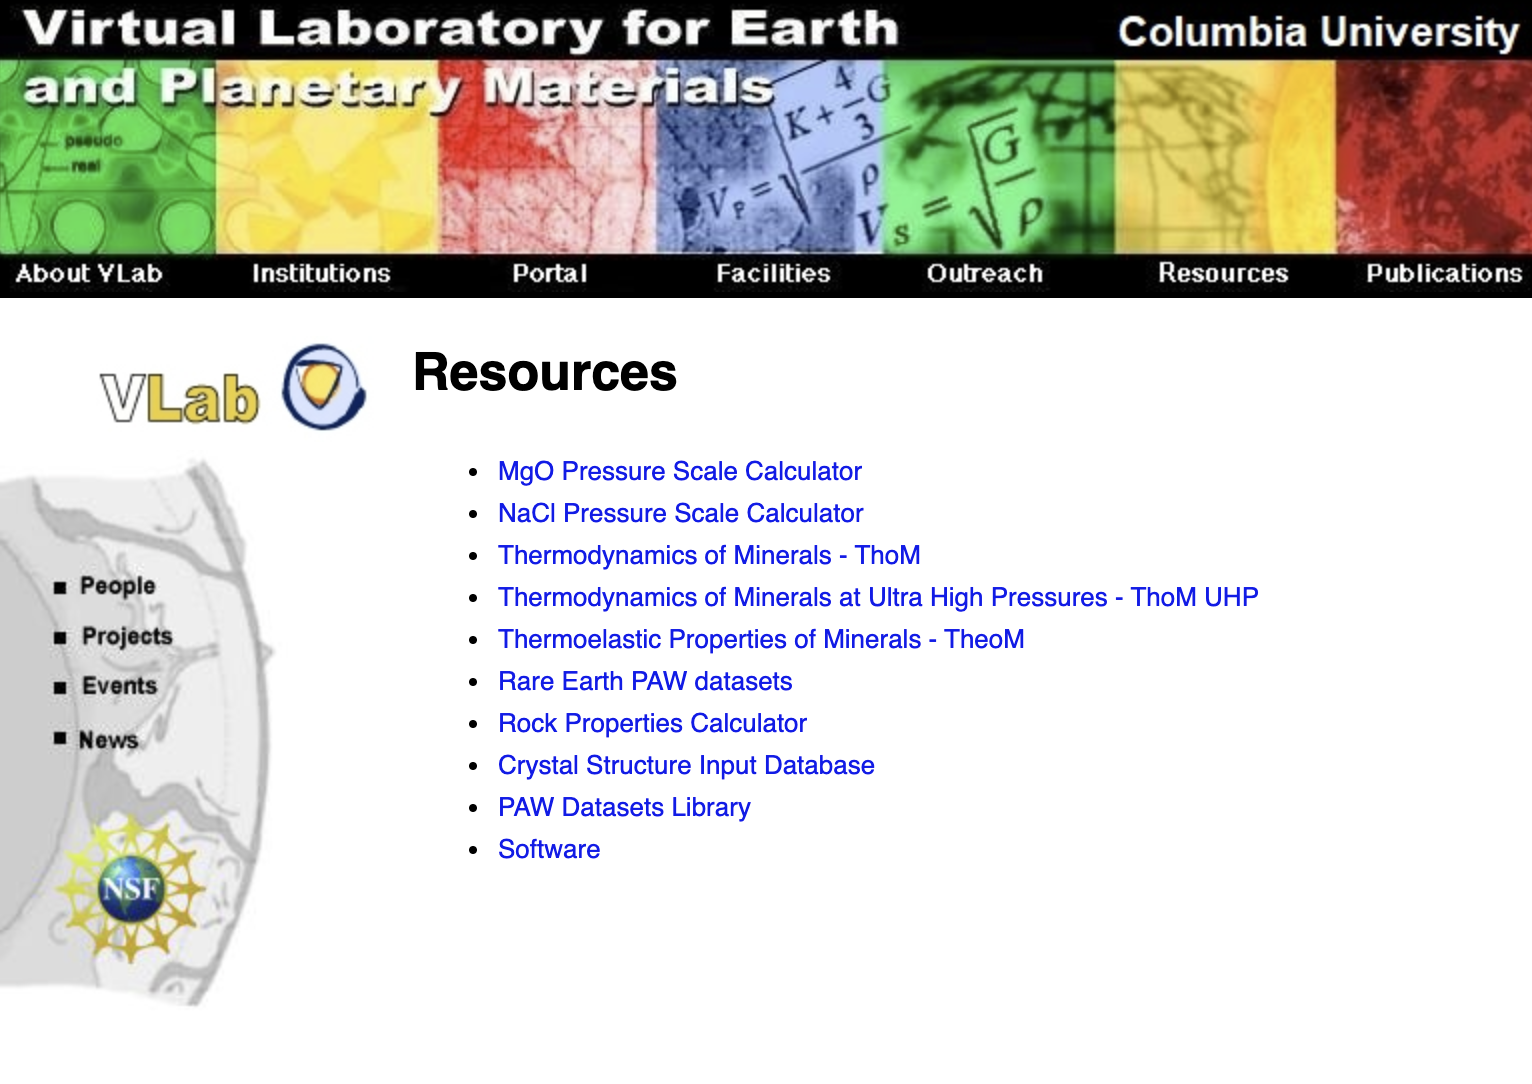
\includegraphics[width=\textwidth]{vlab}
                \caption{\url{http://www.mineralscloud.com/resources/}\footnotemark}
            \end{figure}
        \end{column}
    \end{columns}
    \footcitetext{DASILVA2007321}
\end{frame}
